% LyX 1.5.5 created this file.  For more info, see http://www.lyx.org/.
% Do not edit unless you really know what you are doing.
\documentclass[english,12pt]{revtex4}
\usepackage[T1]{fontenc}
\usepackage[latin9]{inputenc}
\usepackage{nicefrac}
\usepackage{graphicx}

\makeatletter

%%%%%%%%%%%%%%%%%%%%%%%%%%%%%% LyX specific LaTeX commands.
%% Because html converters don't know tabularnewline
\providecommand{\tabularnewline}{\\}

%%%%%%%%%%%%%%%%%%%%%%%%%%%%%% User specified LaTeX commands.
%% LyX 1.5.5 created this file.  For more info, see http://www.lyx.org/.
%% Do not edit unless you really know what you are doing.



\usepackage{nicefrac}


\makeatletter

%%%%%%%%%%%%%%%%%%%%%%%%%%%%%% LyX specific LaTeX commands.
%% Because html converters don't know tabularnewline


%%%%%%%%%%%%%%%%%%%%%%%%%%%%%% User specified LaTeX commands.
%% LyX 1.5.5 created this file.  For more info, see http://www.lyx.org/.
%% Do not edit unless you really know what you are doing.



\usepackage{nicefrac}



\makeatletter

%%%%%%%%%%%%%%%%%%%%%%%%%%%%%% LyX specific LaTeX commands.
%% Because html converters don't know tabularnewline


%%%%%%%%%%%%%%%%%%%%%%%%%%%%%% User specified LaTeX commands.
%% LyX 1.5.5 created this file.  For more info, see http://www.lyx.org/.
%% Do not edit unless you really know what you are doing.



\usepackage{nicefrac}

\begin{document}
\title{{\Large Effect of the Fermi statistics on Thermal Ionization}}

\maketitle

While simulating the ionization equilibrium in partially ionized electron-ion plasmas using Saha 
equations, the electrons are usually assumed to be an ideal Boltzmann gas. 

However, electron is a Fermion with the spin of 1/2. In the practical calculations the condition for
applicability of the Boltzmann gas model for electrons is often not satisfied, resulting in
scarely low accuracy. Therefore, it is worth while checking if one really needs to assume the 
Boltzmann statistics for electrons in solving the ionization equilibrium. 

It appears that 
for realistic quantitative simulations this assumption is not needed at all: to solve the 
ionization equilibrium with the correct Fermi statistics for electrons is not a more difficult problem, 
than that under the incorrect assumption of the Boltzmann statistics.

In a partially ionized plasma, the free electron density corrected by the effects of the Fermi statistics 
('the exchange interaction') should be used in solving the Equation-Of-State (EOS), which is also 
directly affected by the exchange interactions. There is no need to remind that 
{\it at the given electron density} the exchange interaction increases the electron pressure and the 
internal energy density. On the other hand, in partially ionized plasmas this effect may 
be partially or even fully balanced by the electron density decrease due to the exchange interaction 
effect on the ionization equilibrium.  

{\bf Helmholtz free energy.} Consider an ionized monatomic gas with positive non-complex ions. The Helmholtz free energy,
$F=F_{ion}+F_e$, is assumed to be the total of contributions from each of the ion charge states,
$i=0,i_{\max}$ (we apply Eq.(42.3) from \cite{ll} to account for these contributions) as well as the contribution from electrons:
\begin{equation}\label{freeenergy}
F=-T
\sum_{i=0}^{i_{max}}{
N_i\log\left[g_i
             \frac{eV}{N_i}\left(\frac{MT}{2\pi \hbar^2}\right)^{3/2}\exp \left(-\sum_{j=0}^{i-1}\frac{I_j}T \right)\right]}+F_e,
\end{equation}  
where $N_i=n_iV$ is the total number of ions in the charge state $i$ in the volume V,
$I_j$ ($j = 0, 1, 2, \dots$) is the energy needed to ionize an atom or ion from the charge state $j$ to the charge state $j+1$ (the ionization potential).

{\bf Ionization equilibrium: formulation of the problem.} Now we formulate the requirement of the
ionization equilibrium with respect to the reaction $(i)\leftrightarrow(i+1)+e$, for each ion charge state, $i$.
The Helmholtz free energy is a minimum at the equilibrium set of $N_i$ and $N_e$. Therefore, the total
derivative of F with respect to $N_e$ should be zero:
\begin{equation}
\frac{\partial F}{\partial N_e} + \frac{d N_i}{d N_e} \frac{\partial F}{\partial N_i} +
\frac{d N_{i+1}}{d N_e} \frac{\partial F}{\partial N_{i+1}} = 0
\end{equation}
For the reaction under
consideration, the increments in the particle numbers should be 
related as follows: $dN_{i}=-dN_{i+1}=-dN_e$.
Therefore, the requirement, $dF/dN_{i}-dF/dN_{i+1}-dF/dN_e=0$, gives:
\begin{equation}\label{equili}
-T\log\left[\frac{g_{i}}{N_{i}} e^{-\sum_{j=0}^{i-1}I_j/T}\right] + T\log\left[\frac{g_{i+1}}{N_{i+1}} e^{-\sum_{j=0}^{i}I_j/T}\right]-\mu_e=0,
\end{equation}
where we applied the definition of the chemical potential, $\mu=(\partial F/\partial N)_{T,V}$ to the electron gas.
The solution of the ionization equilibrium, hence, reads:
\begin{equation}
N_{i+1}/g_{i+1}=(N_i/g_i)e^{(-\mu_e-I_i)/T},
\end{equation}
or, applying this recursively:
\begin{equation}\label{saharecursive}
N_{i}/g_{i}=(N_0/g_0)e^{(-i\mu_e-\sum_{j=0}^{i-1}I_j)/T}=N_0g_0(g_e)^ie^{-\sum_{j=0}^{i-1}I_j/T},\,\,\,g_e=e^{-\mu_e/T},
\end{equation}
where $g_e$ is the effective "statistical weight" of a free electron.
Indeed, the effective statistical weight of i electrons combined with an ion in the charge state, i, is the
product of statistical weights for each of the particles under consideration, $(g_e)^i g_i$, in accordance with Eq.(\ref{saharecursive})

In the limiting case of $g_e\gg1$ 
(the Boltzmann gas of electrons with negative and large by magnitude value of $\mu_e$) $g_e$ might be interpreted as the
large number of elementary quantum states the detached electron can occupy, which facilitates the ionization by resulting in a higher total probability for 
the ionized state. In the opposite limiting case of degenerate Fermi gas of electrons, the positive chemical potential, $\mu_e>0$, 
tends to the Fermi energy, $E_F$, which in
this limiting case is much greater than the temperature. Accordingly, the exponentially low value of $g_e=e^{-E_F/T}$ in this case means the low 
probability for an electron to jump from a bound state with negative energy to a free state above the threshold of the positive Fermi energy.  

{\bf Partition function and electron density}. We now introduce the ion partition function, $p_i=N_i/N_a$, $N_a$ being 
the total number of atoms. Since the partition function is normalized by unity,
we have:
\begin{equation}
p_i=\frac{g_i(g_e)^ie^{-E_i/T}}S,
\end{equation}
where we introduced the statistical sum:
\begin{equation}
S=\sum_{i=0}^{i_{max}}\left[g_i(g_e)^ie^{-E_i/T}\right]
\end{equation}
as well as the total ionization energy spent to ionize the atom to the state $i$:
\begin{equation}
E_i=\sum_{j=0}^{i-1}I_j
\end{equation}
Introducing also the averaging operator, acting on an arbitrary function of the ion charge number, $\langle f_i\rangle=\sum p_if_i$ and assuming quasi-neutrality, $N_e = \sum{i N_i}$, we
obtain the expression for the electron density:
\begin{equation}\label{zavr}
Z=N_e/N_a=\langle i\rangle.
\end{equation}
On the other hand, for given $T$ and $n_A=N_a/V$ the electron concentration may be found as a function of $g_e(=e^{-\mu_e/T})$.
Now we assume that the electron form an ideal Fermi gas.
This assumption immediately gives us another relationship between the electron density and $g_e$ (see Eq.(56.5) from \cite{ll}):
\begin{equation}\label{zfe}
Z=g_{e1}{\rm Fe}_{1/2}(g_e),
\end{equation}
The coupled equations (\ref{zavr}) and (\ref{zfe}) are used below to solve $Z$ and $g_e$. Herewith
\begin{equation}
g_{e1}(T,N_a/V)=\frac{2V}{N_a}\left(\frac{m_eT}{2\pi \hbar^2}\right)^{3/2}
\end{equation}
is a value such that in the {\it Boltzmann} electron gas $g_e = g_{e1}/Z$ would hold. ${\rm Fe}_\nu(g_e)$ is the Fermi function:
\begin{equation}
{\rm Fe}_\nu(g_e)=\frac1{\Gamma(\nu+1)}\int{\frac{x^\nu dx}{g_ee^x+1}},
\end{equation}
where $\Gamma$-function is introduced as usually: $\Gamma(\nu+1)=\nu \Gamma(\nu),\,\Gamma(1/2)=\pi^{1/2}$.
Below we use the following auxiliary functions:
\begin{equation}
R^-(g_e)=\frac{{\rm Fe}_{-1/2}(g_e)}{{\rm Fe}_{1/2}(g_e)}, \qquad
R^+(g_e)=\frac{{\rm Fe}_{3/2}(g_e)}{{\rm Fe}_{1/2}(g_e)}.
\end{equation}
Detailed discussion on the Fermi functions is delegated to the Appendix.

{\bf To solve the ionization equilibrium} for the given $T$ and $n_a=N_a/V$, one needs to solve $g_e$ from equation $G(g_e)=0$, 
$G(g_e)=\langle i\rangle-g_{e1}{\rm Fe}_{1/2}(g_e)$, which is obtained by means of excluding $Z$ from Eqs.(\ref{zavr},\ref{zfe}). 
It may be solved using the Newton-Rapson iterations: with any trial value, $\log(g_e)_{old}$, the improved value, $\log(g_e)_{new}$, 
is obtained from the equation as follows:
\begin{equation}\label{iter}
\log(g_e)_{new}=%\log(g_e)_{old}-\frac{G((g_e)_{old})}{G^\prime((g_e)_{old})}=
\log(g_e)_{old}-\frac{\langle i\rangle-g_{e1}{\rm Fe}_{1/2}((g_e)_{old})}{
\langle i^2\rangle-\langle i\rangle^2+ Z R^-((g_e)_{old}) },
\end{equation}
where the derivative $g_eG^\prime$, which should stand in the denominator in 
Eq.(\ref{iter}) is derived using the easy-to-check equations as follows:
\begin{equation}
g_e\frac{d{\rm Fe}_\nu(g_e)}{dg_e}=-{\rm Fe}_{\nu-1}(g_e),
\end{equation}
and, for any set of values in the charge states, $f_i$:
\begin{equation}
g_e\frac{\partial\langle f_i\rangle}{\partial g_e}=\langle if_i\rangle-\langle f_i\rangle\langle i\rangle
\end{equation}

We see that to solve iterations in Eq.(\ref{iter}) for Fermi gas of electrons is not
more computationally intense problem as compared to the same procedure by assuming electrons 
to be the Boltzmann gas. In the latter case, $g_e \to +\infty$, we have $Fe_\nu(g_e) \approx 1/g_e$
(see Eq.(\ref{feboltzmann}) below) and $g_e \approx g_{e1}/Z$, which allows us to iterate Eq.(\ref{iter})
as a somewhat simpler equation for $Z$:
$\log (Z_{new})=\log(Z_{old})+(\langle i\rangle-Z_{old})/(Z_{old}+\langle i^2\rangle-\langle i\rangle^2)$. However, in any case the most cumbersome computations 
while solving Eq.(\ref{iter}), for Fermi gas, or the equation for $Z$, for Boltzmann gas, is in calculating, although explicitly, the 
numerous partition functions for many charge
states and excitation levels. Compared with these bulk computations, the presence of the Fermi functions in Eq.(\ref{iter}), which may be tabulated 
for all interesting cases of $\nu=-1/2,1/2,3/2$, % as well as a single inverse function, ${\rm Fe}^{-1}_{1/2}$ 
does not matter at all.

Therefore, we 
do not see any reason for applying the assumption of the Boltzmann electron gas in modelling the ionization equilibrium
in real dense plasmas.

{\bf Derivatives along the ionization curve.}
Taking differential of the equation of ionization equilibrium, $G=0$, one gets the equation relating the differentials
of different variables along the curve of ionization equilibrium:
\begin{equation}\label{diffge}
\frac{dg_e}
{g_e}
\left(
\langle i^2\rangle-Z^2+ZR^-(g_e)
\right)+\frac{dT}{T^2}
\left(\langle iE_i\rangle-\langle E_i\rangle Z)\right)=\left(\frac32\frac{dT}{T}+\frac{dV}V\right)Z,
\end{equation}
herewith we substitute wherever possible $Z$ for $\langle i\rangle$ and $g_{e1}{\rm Fe}_{1/2}(g_e)$.
Accordingly, the differential of $Z$ is:
\begin{equation}\label{diffz}
dZ=\left(\frac32\frac{dT}{T}+\frac{dV}V-\frac{R^-(g_e)dg_e}{g_e}\right)Z
\end{equation}

{\bf Estimate the effect of the Fermi statistics on the ionization degree.}
Eqs.(\ref{diffge},\ref{diffz}) allow us to evaluate the effect of electron Fermi statistics on ionization.
From Eq.(\ref{feboltzmann}) one can
see that for large $g_e$ (Boltzmann gas) the equation, $G(g_e)=0$, reduces to $\langle i\rangle-g_{e1}/g_e=\delta_{\rm Fe}$,
where $\delta_{\rm Fe}$ is a small negative correction to the Fermi function at $g_e \to \infty$:
\begin{equation}\label{feboltzmann}
Fe_\nu(g_e)=\frac{1}{\Gamma(\nu+1)} \int \frac{x^\nu dx}{g_e e^x + 1} =
\frac{1}{\Gamma(\nu+1)} \int \frac{x^\nu dx}{g_e e^x} + \delta_{\rm Fe} = \frac{1}{g_e} + \delta_{\rm Fe}.
\end{equation}
%Considering $\delta_{\rm Fe}$ negligible, one can find $g_e=g_{e1}/Z$ from Eq.(\ref{zfe})

Then assuming $\delta_{\rm Fe}$ to be a small increment in the right hand side of Eqs.(\ref{diffge},\ref{diffz}) and by
finding $dg_e/\delta_{\rm Fe}$ from Eq.(\ref{diffge}) at $dV=dT=0$ and then find $dZ/\delta_{\rm Fe}$ from Eq.(\ref{diffz}):
\begin{equation}
\delta Z=Z\delta_{\rm Fe}\frac{\langle i^2\rangle-Z^2}{\langle i^2\rangle-Z^2+Z}. 
\end{equation}
The correction is negative as long as $\delta_{\rm Fe}$ is negative. Thus, due to the Fermi gas effects for detached electrons, the ionization degree is
always lower than that predicted by the Saha equilibrium equations under assumption of the Boltzmann electron gas.

This effect should be accounted for while
treating the effect of the Fermi statistics for electrons in the equation of state. Specifically, {\it at constant electron density} the exchange interactions 
between the electrons increases the electron pressure, but in the partially ionized plasma the magnitude (if not the sign!) of this effect can be  
compromised by the pressure reduction due to the decrease in the electron density. 

{\bf Plasma thermodynamics and Equation-Of-State.} Now we substitute the ion partition function to Eq.(\ref{freeenergy}). After some algebra we obtain:
\begin{equation}\label{equile}
F = -TN_a\log\left[\frac{eV}{N_a}\left(\frac{MT}{2\pi \hbar^2}\right)^{3/2}\right]-TN_a\log S +\Omega_e,
\end{equation}
the thermodynamic potential $\Omega_e=F_e -\mu_eZN_a$ for Fermi gas of electrons is given by Eq.(56.6) from \cite{ll}:
\begin{equation}
\Omega_e = -[g_{e1}N_a]T{\rm Fe}_{3/2}(g_e),
\end{equation}
the product in the square brackets being actually independent of $N_a$, because $g_{e1}\sim N_a^{-1}$. Eq.(\ref{equile}) provides the free energy in the case of
local thermodynamic equilibrium with the first term being the contribution from the ion translational energy. This term may be written as the function of the ion 
temperature, in the case the latter differs from the electron one. Unless the ion-ion interaction is taken into account, this first term gives the contributions 
of $n_aT_i$ and $3n_aT_i/2$ to the total plasma pressure and total energy density correspondingly. The second term is
the Boltzmann distribution of ions over the ionization and excitation states, expressed in terms of the statistical sum. Finally, the electron gas with the
variable particle number gives the contribution of $\Omega_e$ instead of $F_e$. 

While differentiating Eq.(\ref{equile}) with respect to $T$ and $V$, it is important that the derivatives
by $g_e$ from the second and third terms cancel 
each other: $g_e(\partial \log S/\partial g_e)=\langle i\rangle=Z$ and $-g_eg_{e1}{\rm Fe}^\prime_{3/2}(g_e)=g_{e1}{\rm Fe}_{1/2}=Z$. That is why for the internal energy density, 
${\cal E}$, and for the pressure we find:
\begin{equation}
{\cal E} = -\frac{T^2}V\left(\frac{\partial}{\partial T}\left(\frac F T\right)\right)=
{\cal E}_i+{\cal E}_e,\qquad{\cal E}_i=\frac32Tn_a,
\qquad{\cal E}_e=n_a\left[\frac32TZR^+(g_e)+\langle E_i\rangle\right],
\end{equation}
\begin{equation}
P = -\frac{\partial F}{\partial V}=P_i+P_e,\qquad
P_i = n_aT,\qquad
P_e = n_aTZR^+(g_e).
\end{equation}

However, while calculating the second order thermodynamic derivatives, like the specific heat, the derivatives of $g_e$ essentially sophisticate the 
calculations. The result may be expressed in terms of covariances: $\langle\delta^2i\rangle=\langle(i-Z)^2\rangle$, $\langle\delta^2E\rangle=\langle(E_i-\langle E_i\rangle)^2 \rangle$ and 
$\langle\delta i\delta E\rangle=\langle(E_i-\langle E_i\rangle)(i-Z)\rangle$. In such a way one can find the specific heat in isochoric process, per the unit of volume:
\begin{equation}
C_{Ve}=\frac{\partial {\cal E}_e}{\partial T}=n_a\left[\frac{\langle\delta^2E\rangle}{T^2}+\frac{15}4ZR^+
-\frac{\left(\frac32Z-\frac{\langle\delta E\delta i\rangle}T\right)^2}{\langle\delta^2i\rangle+ZR^-}\right],
\end{equation}
the temperature derivative of pressure:
\begin{equation}
\frac {\partial P_e}{\partial T}=n_aZ\left[\frac52 R^+ -\frac{\frac32Z-\frac{\langle\delta E\delta i\rangle}T}{\langle\delta^2i\rangle+ZR^-}\right],
\end{equation}
as well as the isothermal compressibility:
\begin{equation}
V\frac{\partial P_e}{\partial V}=-\frac{Z^2n_aT_e}{\langle\delta^2i\rangle+ZR^-},
\end{equation}
for simplicity in the above equations the contributions due to ion translational motions are omitted, which are:
\begin{equation}
C_{Vi}=\frac32n_a, \qquad
\frac{\partial P_i}{\partial T}=n_a, \qquad
V\frac{\partial P_i}{\partial V}=-n_aT.
\end{equation}

%  Copyright (C) 2002 Regents of the University of Michigan, portions used with permission 
%  For more information, see http://csem.engin.umich.edu/tools/swmf

\section{Appendix A: The Fermi function calculation approach}

For $g_e\ge1,\,\nu>-1$ the Fermi function may be developed into
convergent power series (see Eq.(5) from \cite{mcleod}):
\begin{equation}
{\rm Fe}_\nu(g_e)=\sum_{n=1}^\infty{\frac{(-1)^{n+1}}{n^{\nu+1}(g_e)^n}}.
\end{equation} 

The Taylor series in powers of $-\log(g_e)$ (see Eq.(6) from \cite{mcleod}): % from MacLeod
\begin{equation}
{\rm Fe}_{\nu}(g_e) = \sum_{i=0}^\infty{\frac{(1-2^{i-\nu}) \zeta(\nu+1-i)}{i!} (-\log(g_e))^i}.
\end{equation}
is only used for $g_e \in [e^{-3}; 1)$, because it converges when $|\log(g_e)| < \pi$.

For $0 < g_e < e^{-3}$ we use the following asymptotic series (see Eq.(8) from \cite{mcleod}): % from MacLeod
\begin{equation}
{\rm Fe}_{\nu}(g_e) \sim \frac{(-\log(g_e))^{\nu+1}}{\Gamma(k+2)} \left(1 + \sum_{i=1}^\infty{a_{2i} (\log(g_e))^{-2i}}\right).
\end{equation}
where
\begin{equation}
a_{2i} = \frac{(1 - 2^{1-2i})(k+1)!(2\pi)^{2i}}{(k+1-2i)!} \frac{|B_{2i}|}{(2i)!}.
\end{equation}
where $B_j$ denotes a standard Bernoulli number. The last formula can be simplified using the following expression for the Bernoulli numbers (see Eq.(9.616) from \cite{gradshtein}):
\begin{equation}
B_{2i} = \frac{(-1)^{i-1} (2i)!}{2^{2i-1} \pi^{2i}} \zeta(2i).
\end{equation}
so that
\begin{equation}
a_{2i} = \frac{2 (1 - 2^{1-2i}) (k+1)!}{(k+1-2i)!} |\zeta(2i)|.
\end{equation}

We only calculate the first three sum terms of the asymptotic series to get the best
approximation of ${\rm Fe}_\nu(g_e)$ for $g_e$ around $e^{-3}$:
\begin{equation}
{\rm Fe}_\nu(g_e) \approx \frac{(-\log(g_e))^{\nu+1}}{\Gamma(k+2)} \left(1 + \frac{a_2}{(\log(g_e))^2} + \frac{a_4}{(\log(g_e))^4}\right).
\end{equation}
An  asymptotic series does not guarantee an improvement in accuracy while increasing the number of the sum terms
involved. In our particular case the use of either more than or less than three sum
terms noticeably lowers the accuracy of ${\rm Fe}_\nu(g_e)$ for $g_e \in [e^{-5}, e^{-3}]$.

In both series $\zeta(x)$ denotes the Riemann zeta-function.
At $x > 0$ it can be calculated as a convergent series (see Eq.(9.522.2) from \cite{gradshtein}): % Gradshtein, Ryzhik: 9.522.2; Abramowitz: 23.2.19
\begin{equation}
\zeta(x) = \frac{1}{1-2^{1-x}} \sum_{n=1}^\infty{(-1)^{n+1} \frac{1}{n^x}}.
\end{equation}
At $x < 0$ we use the following reflection formula (see Eq.(7) from \cite{mcleod}): % MacLeod
\begin{equation}
\zeta(x) = 2^x \pi^{x-1} \sin(\frac{\pi x}{2}) \Gamma(1-x) \zeta(1-x).
\end{equation}

\begin{figure}[ht]
\centering
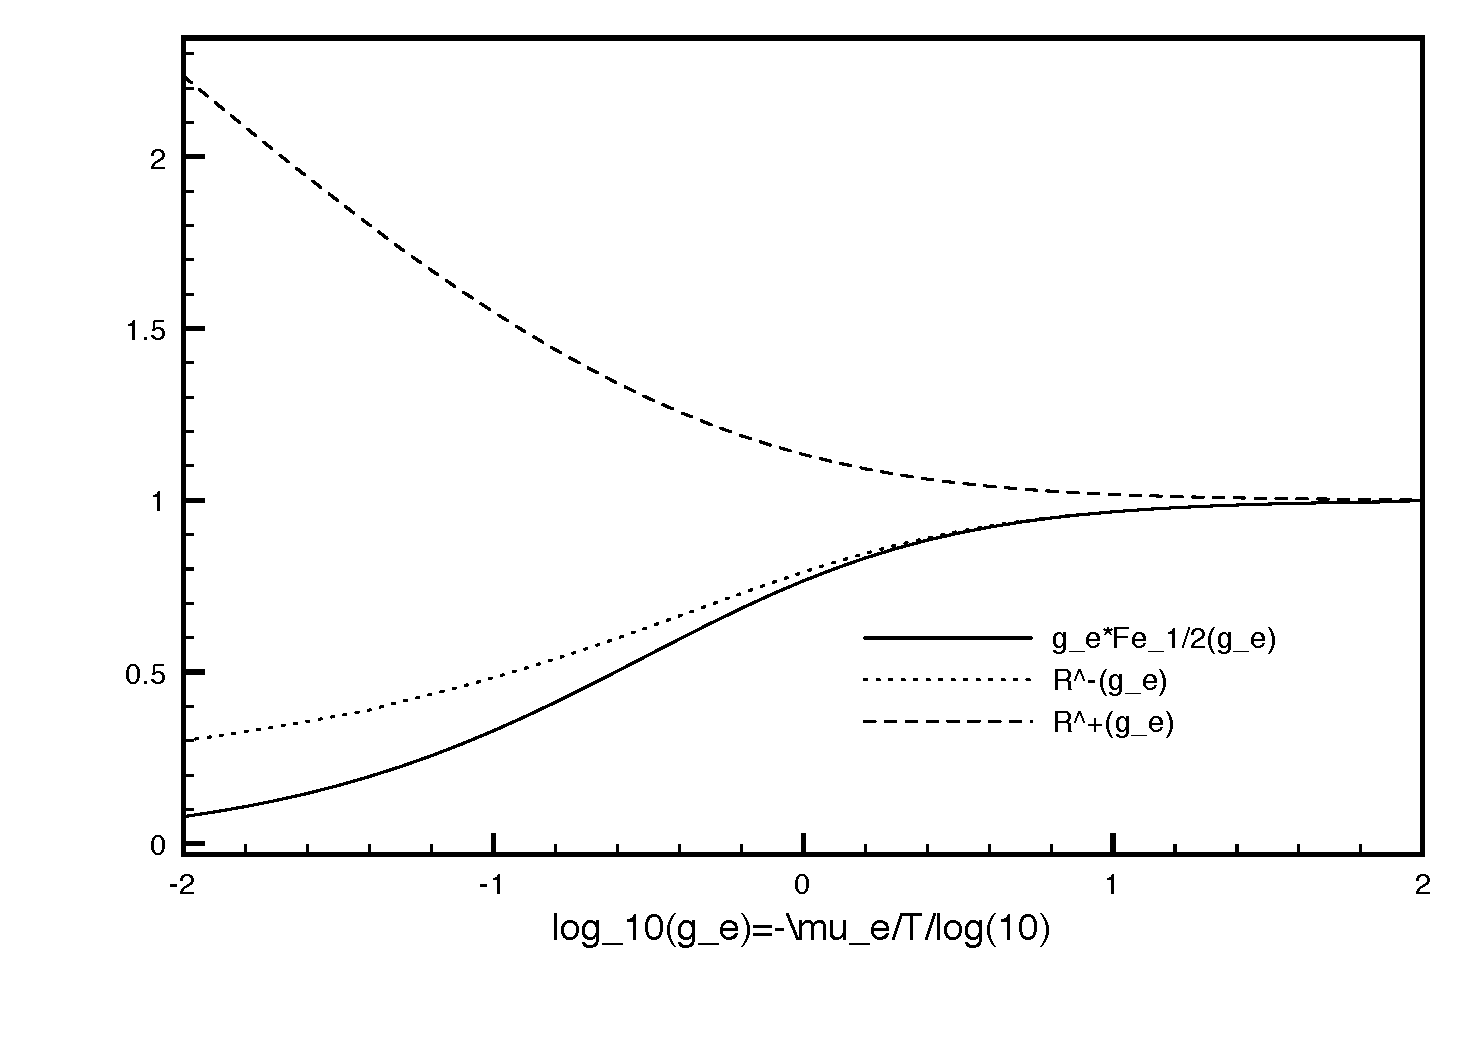
\includegraphics[scale=0.6]{FermiFunction.eps}
\caption{The Fermi function of index 1/2 multiplied by $g_e$ (solid) and the ratio functions (dashed) calculated using the described algorithm.}
\end{figure}


%\include{CoulombInteraction}


%{\bf Conclusion.} Again, mention that in the partially ionized plasma the exchamge interaction
%effect on the plasma pressure is not exhausted by the multiplier  $R^+\ge 1$, there is also the reduction in $Z$ proportional to negative 
%$\delta_{\rm Fe}$. This thermodynamical property of the partial ionized gas should be also taken into account while 
%generalizing the result for the case of small but finite Coulomb interactions, which may be  done by developing the
%chemical potential of the electron gas into a series of the average Coulomb potential of electrons.   

\begin{thebibliography}{99}
\bibitem{ll}
L.D.Landau and E.M.Lifshitz, Theoretical Physics. Vol.5. Statistical Physics, Part 1. 3rd Edition. Pergamon Press, NY, 1980.
%\bibitem{PD}
%R.P.Drake, High-Energy-Density Physics,
%\bibitem{DS}
%D.Saltman, Atomic Physics in Hot Plasmas, Oxford University Press US, 1998
\bibitem{gradshtein}
I.S.Gradshteyn and I.M.Ryzhik, Table of Integrals, Series and Products. Academic Press, NY, 1965.
\bibitem{mcleod}
A.J.MacLeod, Algorithm 779: Fermi-Dirac Functions of Order -1/2, 1/2, 3/2, 5/2. ACM Transactions on Mathematical Software, Vol. 24, No. 1, March 1998.
\end{thebibliography}
\end{document}
Ignore the formula below, we will need it later:
\begin{equation}
F=T \log \left[\sum_{i=0}^Zg^i\exp\left(-\frac{\sum_{j=0}^iI_j}T\right)\right],\,\,\,\,\,\,g\sim\frac{T^{3/2}}{N_e}.
\end{equation}

